\documentclass{report}
\usepackage[utf8]{inputenc}
\usepackage{CJKutf8}
\usepackage{amsmath}
\usepackage{tikz-qtree}
\usepackage{pgfplots}
\usepackage{hyperref}
\usepackage{graphicx}
\usepackage{cases}
\usetikzlibrary{trees}
\title{ネットワーク設計論レポート1}
\author{27019679 グレゴリウスブライアン}
\setlength{\parindent}{0pt}

\begin{document}
\begin{CJK}{UTF8}{min}
    \maketitle
    \newpage
    \section*{演習3 問題1}
    \begin{figure}[h!]
        \centerline{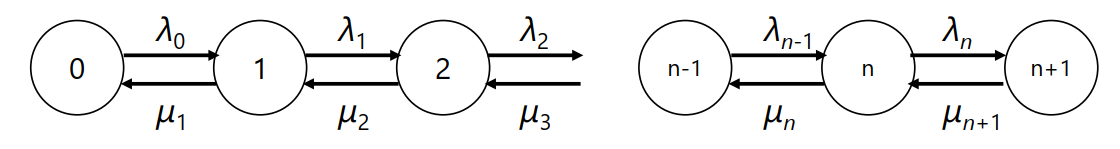
\includegraphics[width=\linewidth]{1.png}}
        \caption{待ち行列$M/M/1 (\infty)$と$M/M/c (\infty)$の状態遷移図}
    \end{figure}
    Figure 1で与えられたような待ち行列モデルを考える。このとき、\\
    系内人数が$n$という状態の潜在確率を$p_n$\\
    系内人数が$n$のときの新しい客の到着率を$\lambda_n$\\
    系内人数が$n$のときのサービスを終えた客の離脱率を$\mu_n$\\
    同時に来れる客が1人に限るとする。
    定常状態では、すべての状態に対して、遷移確立が均衡である。
    このため各状態について、次の平衡方程式が成り立つ:

    \begin{numcases}{}
        p_0\lambda_0=p_1\mu_1 & $n=0$  \\
        (\lambda_n+\mu_n)p_n=p_{n+1}
        \mu_{n+1}+p_{n-1}\lambda_{n-1}&$n\neq0$
    \end{numcases}

    また、システムの状態は常にどれか一つの状態にあるため、
    \begin{equation}
        \sum_{n=0}^\infty p_n=1
    \end{equation}

    式$(1)$を$p_1$について解くと次になる。
    \begin{equation}
        p_1=\frac{\lambda_0}{\mu_1}p_0
    \end{equation}
    次に$(2)$の式の左側の$p_n$を$p_1$とすると$(4)$を用いて、$p_2$について解く:
    \begin{equation}
        \begin{aligned}[b]
            (\lambda_1+\mu_1)p_1                        & =p_{2}\mu_{2}+p_{0}\lambda_{0}                                 \\
            (\lambda_1+\mu_1)\frac{\lambda_0}{\mu_1}p_0 & =p_{2}\mu_{2}+p_{0}\lambda_{0}                                 \\
            p_{2}\mu_{2}                                & =\frac{\lambda_0\lambda_1}{\mu_1}p_0+\lambda_0p_0-\lambda_0p_0 \\
            p_{2}                                       & =\frac{\lambda_0\lambda_1}{\mu_1\mu_{2}}p_0
        \end{aligned}
    \end{equation}
    これより、一般の$n$に対して次が成り立つ
    \begin{equation}
        p_n=\frac{\lambda_0\lambda_1\cdots\lambda_{n-1}}{\mu_1\mu_2\cdots\mu_n}p_0
    \end{equation}
    式$(3)$を変形し、$(6)$を代入すれば$p_0$が決まる
    \begin{equation}
        \begin{aligned}[b]
            \sum_{n=0}^\infty p_n                                                                                    & =1                                                                                                 \\
            p_0+\sum_{n=1}^\infty \frac{\lambda_0\lambda_1\cdots\lambda_{n-1}}{\mu_1\mu_2\cdots\mu_n}p_0             & =1                                                                                                 \\
            p_0\left( 1+\sum_{n=1}^\infty \frac{\lambda_0\lambda_1\cdots\lambda_{n-1}}{\mu_1\mu_2\cdots\mu_n}\right) & =1                                                                                                 \\
            p_0                                                                                                      & =\frac{1}{1+\sum_{n=1}^\infty \frac{\lambda_0\lambda_1\cdots\lambda_{n-1}}{\mu_1\mu_2\cdots\mu_n}}
        \end{aligned}
    \end{equation}


    \newpage
    \section*{演習3 問題2:$M/M/1$ 状態確率}
    $M/M/1$について各状態$p_n$と$p_0$の関係を調べる。
    $M/M/1(\infty)$では$\lambda_0=\lambda_1=\dots=\lambda, \mu_0=\mu_1=\dots=\mu$なので利用率$\rho=\lambda/\mu$と仮定すれば式$(6)$と$(7)$は次のようにあらわせる
    \begin{equation}
        p_n=\rho^n p_0
    \end{equation}
    \begin{equation}
        \begin{aligned}[b]
            p_0 & =\frac{1}{1+\sum_{n=1}^\infty \rho^n}
        \end{aligned}
    \end{equation}
    分母にある和は初項$\rho$公比$\rho$の等比数列であり、その和は等比数列の和の公式により次のように求められる。
    \begin{equation}
        \begin{aligned}[b]
            \sum_{n=1}^\infty \rho^n & =\lim_{n\to\infty}\frac{\rho(\rho^n-1)}{\rho-1} \\
        \end{aligned}
    \end{equation}
    まず、$0<\rho<1$について議論する。
    このとき、式$(10)$は次になる:
    \begin{equation}
        \begin{aligned}[b]
            \sum_{n=1}^\infty \rho^n & =\frac{\rho}{1-\rho} \\
        \end{aligned}
    \end{equation}
    $(9)$に$(11)$を代入すれば$p_0$が次のように表現できる。
    \begin{equation}
        \begin{aligned}[b]
            p_0 & =\frac{1}{1+\frac{\rho}{1-\rho}} \\
            p_0 & =1-\rho
        \end{aligned}
    \end{equation}
    $(12)$を$(8)$に入れたら次の関係式が成り立つことがわかる
    \begin{equation}
        p_n=\rho^n (1-\rho)
    \end{equation}
    次に$\rho\geq1$の時を考える。このとき、式$(9)$の右辺の分母が正の無限大に発散するので、$p_0$が$0$に収束する。
    $\rho\geq1$は待ち行列長がどんどん長くなると解釈できる。このとき、$p_0=0$はつまり、系内人数が0になる(お客さんが対応し切れる)ことがないと解釈できる。
    今回の解析は系内人数が無限大である想定の解析であるため、$\rho\geq1$のとき、式$(9)$の分母が式$(8)$の$p_0$の係数よりも大きくなるため、
    各$n$について$p_n$は常に微小な値になってしまうという不思議な現象が起こる(行列が無限に長くなる)。しかし、実際最大系内人数に実際に指定すれば、呼損率が大きくなるがきちんとした$p_n$や$p_0$の計算ができる。

    \newpage

    \section*{演習3 問題3:$M/M/c$ 状態確率}
    次に、$M/M/c$について各状態$p_n$と$p_0$の関係を調べる。
    $M/M/c(\infty)$についてを考える。このとき、次の関係が成り立つ
    \begin{equation}
        \lambda_0=\lambda_1=\dots=\lambda
    \end{equation}
    \begin{numcases}{\mu_n}
        n\mu & $(n=0,1,2,\dots,c-1)$\\
        c\mu & $(n=c,c+1,\dots)$
    \end{numcases}
    $\rho=\frac{\lambda}{c\mu}$と置いて、$(15)$と$(16)$を式$(7)$に代入すると
    \begin{equation}
        \begin{aligned}[b]
            p_0 & =\frac{1}{1+\sum_{n=1}^{c-1} \frac{\lambda^n}{(1\mu)(2\mu)\cdots (n\mu)}+\sum_{n=c}^\infty \frac{\lambda^n}{(1\mu)(2\mu)\cdots (c-1\mu)(c\mu)\cdots(c\mu)}}                       \\
            p_0 & =\frac{1}{1+\sum_{n=1}^{c-1} \frac{\lambda^n}{n!\mu^n} +\sum_{n=c}^\infty \frac{\lambda^{n-c}}{(c\mu)^{n-c}} \cdot \frac{\lambda^{c}}{(c)!\mu^{c}}}                               \\
            p_0 & =\frac{1}{1+\sum_{n=1}^{c-1} \frac{\lambda^n}{\frac{n!}{c^n}c^n\mu^n} +\sum_{n=c}^\infty \frac{\lambda^{n-c}}{(c\mu)^{n-c}} \cdot \frac{\lambda^{c}}{\frac{(c)!}{c^c}c^c\mu^{c}}} \\
            p_0 & =\frac{1}{1+\sum_{n=1}^{c-1} \frac{(c\rho)^n}{n!} + \frac{(c\rho)^c}{c!} \sum_{n=c}^\infty \rho^{n-c} }                                                                           \\
        \end{aligned}
    \end{equation}
    ここで再び$0<\rho<1$の仮定で議論する。式(17)の分母の和の部分は初項 $1$、公比 $\rho$ 無限等比級数である。そのため、等比数列の和の公式を利用して次の関係式が成り立つ。
    \begin{equation}
        \begin{aligned}[b]
            \sum_{n=0}^\infty \rho^n & =\lim_{n\to\infty}\frac{(\rho^n-1)}{\rho-1} \\
            \sum_{n=0}^\infty \rho^n & =\frac{1}{1-\rho}                           \\
        \end{aligned}
    \end{equation}
    式$(17)$に式$(18)$を代入すると$p_0$の値が決まる
    \begin{equation}
        \begin{aligned}[b]
            p_0 & =\frac{1}{1+\sum_{n=1}^{c-1} \frac{(c\rho)^n}{n!} + \frac{(c\rho)^c}{c!(1-\rho)}} \\
        \end{aligned}
    \end{equation}
    同様に、$(15)$と$(16)$で$(6)$を表すと次の$p_n$と$p_0$の関係式が成り立つ
    \begin{numcases}{p_n=}
        \frac{\lambda^n}{n!\mu^n}p_0 & $n=1,2,\dots,c-1$\\
        \frac{\lambda^n}{(c)!\mu^c c^{n-c} \mu^{n-c}}p_0 & $n=c,c+1,\dots$
    \end{numcases}
    $\rho$を用いると$(20)$と$(21)$は次のように表せる
    \begin{numcases}{p_n=}
        \frac{(c\rho)^n}{n!}p_0 & $n=1,2,\dots,c-1$\\
        \frac{c^c}{c!}\rho^np_0 & $n=c,c+1,\dots$
    \end{numcases}

    \newpage
    \section*{演習4 問題1:$M/M/c$ 平均行列長}
    $M/M/c$の平均待ち行列長$L_q$は系内人数$n$が$c+1$以上である各の状態に対して$n-c$(行列にいる人の数)に関する期待値である。
    \begin{equation}
        L_q=\sum_{n=c+1}^\infty (n-c)p_n
    \end{equation}
    式$(23)$より、
    \begin{equation}
        \begin{aligned}[b]
            L_q & =\sum_{n=c+1}^\infty (n-c)\frac{c^c}{c!}\rho^np_0          \\
                & p_0\frac{c^c\rho^c}{c!}\sum_{n=c+1}^\infty (n-c)\rho^{n-c}
        \end{aligned}
    \end{equation}
    $k=n+c$と置くと
    \begin{equation}
        L_q=p_0\frac{c^c\rho^c}{c!}\sum_{k=1}^\infty k\rho^k
    \end{equation}
    次に、項別微分によって次が表せる。
    \begin{equation}
        \begin{aligned}[b]
            \frac{\partial}{\partial\rho}\sum_{k=0}^{\infty}\rho^k & =\sum_{k=0}^{\infty}\frac{\partial}{\partial\rho}\rho^k     \\
            \frac{\partial}{\partial\rho}\sum_{k=0}^{\infty}\rho^k & =\sum_{k=0}^{\infty}k\rho^{k-1}                             \\
            \frac{\partial}{\partial\rho}\sum_{k=0}^{\infty}\rho^k & =\frac{1}{\rho}\sum_{k=0}^{\infty}k\rho^{k}                 \\
            \sum_{k=0}^{\infty}k\rho^{k}                           & =\rho\frac{\partial}{\partial\rho}\sum_{k=0}^{\infty}\rho^k
        \end{aligned}
    \end{equation}
    式(27)の左辺の和は$k=0$の時$0$になるので次のように書ける
    \begin{equation}
        \begin{aligned}[b]
            \sum_{k=1}^{\infty}k\rho^{k} & =\rho\frac{\partial}{\partial\rho}\sum_{k=0}^{\infty}\rho^k
        \end{aligned}
    \end{equation}
    式(26)、(28)より、
    \begin{equation}
        L_q=p_0\frac{c^c\rho^c}{c!}\rho\frac{\partial}{\partial\rho}\sum_{k=0}^{\infty}\rho^k
    \end{equation}
    $0<\rho<1$を仮定し、(18)より、
    \begin{equation}
        \begin{aligned}[b]
            L_q & =p_0\frac{c^c\rho^c}{c!}\rho\frac{\partial}{\partial\rho}\left(\frac{1}{1-\rho}\right) \\
            L_q & =p_0\frac{(c\rho)^c}{c!}\rho\frac{1}{(1-\rho)^2}
        \end{aligned}
    \end{equation}
    $\rho$について整理すると、
    \begin{equation}
        L_q=\frac{\rho}{1-\rho}b
    \end{equation}
    ただし、
    \begin{equation}
        b=\frac{(c\rho)^c}{c!(1-\rho)}p_0
    \end{equation}
    この$b$は
    \begin{equation}
        b=\sum_{n=c}^\infty p_n=\frac{(c\rho)^c}{c!(1-\rho)}p_0
    \end{equation}
    つまり、待ち行列がすべてふさがっている確率であること同じことになる。

    \newpage
    \section*{演習4 問題2:$M/M/c$ 平均系内人数}
    $M/M/c$ 平均系内人数は次の式で与えられる
    \begin{equation}
        \begin{aligned}[b]
            L & =\sum_{n=0}^{\infty}np_n                                                    \\
            L & =\sum_{n=c+1}^{\infty}(n-c)p_n+\sum_{n=c+1}^{\infty}cp_n+\sum_{n=1}^{c}np_n
        \end{aligned}
    \end{equation}
    式(34)の右辺の第1項は平均待ち行列長であり、式(31)で与えられる。第2項は待ち行列があるときの窓口にある人数、第3項は待ち行列がないときの系内人数。
    まず、待ち行列があるときの窓口にある人数について考える。式(23),(33)より、
    \begin{equation}
        \begin{aligned}[b]
            \sum_{n=c+1}^{\infty}cp_n & =\sum_{n=c+1}^{\infty}c\frac{c^c}{c!}\rho^np_0          \\
                                      & =c\rho\sum_{n=c+1}^{\infty}c\frac{c^c}{c!}\rho^{n-1}p_0 \\
                                      & =c\rho\sum_{n=c+1}^{\infty}p_{n-1}                      \\
                                      & =c\rho\sum_{n=c}^{\infty}p_n                            \\
                                      & =c\rho b
        \end{aligned}
    \end{equation}
    次に、待ち行列がないときの系内人数は式(22)より、
    \begin{equation}
        \begin{aligned}[b]
            \sum_{n=1}^{c}np_n & =\sum_{n=1}^{c}n\frac{(c\rho)^n}{n!}p_0               \\
                               & =\sum_{n=1}^{c}\frac{c\rho(c\rho)^{(n-1)}}{(n-1)!}p_0 \\
                               & =c\rho\sum_{n=1}^{c}p_{n-1}                           \\
                               & =c\rho\sum_{n=0}^{c-1}p_{n}
        \end{aligned}
    \end{equation}
    (3),(33)より、
    \begin{equation}
        \begin{aligned}[b]
            \sum_{n=0}^{c-1}p_{n}+\sum_{n=c}^{\infty}p_{n} & =1 \\
            \sum_{n=0}^{c-1}p_{n}+b=1                           \\
            \sum_{n=0}^{c-1}p_{n}=1-b
        \end{aligned}
    \end{equation}
    (36),(37)より、
    \begin{equation}
        \begin{aligned}[b]
            \sum_{n=1}^{c}np_n & =c\rho(1-b)
        \end{aligned}
    \end{equation}
    式(34)に(31),(35),(38)を代入すると、
    \begin{equation}
        \begin{aligned}[b]
            L & =L_q+c\rho b+c\rho (1-b) \\
            L & =L_q+c\rho
        \end{aligned}
    \end{equation}

    \newpage
    \section*{演習4 問題3:$M/M/c$実値計算例}
    一旦$M/M/c$についてすべての式をまとめる。\\
    平均待ち行列長:
    \begin{equation}
        L_q=\frac{\rho}{1-\rho}b
    \end{equation}
    平均系内人数:
    \begin{equation}
        \begin{aligned}[b]
            L & =L_q+c\rho
        \end{aligned}
    \end{equation}
    平均待ち時間:
    \begin{equation}
        W_q=\frac{L_q}{\lambda}=\frac{b}{c\mu(1-\rho)}
    \end{equation}
    平均系内時間:
    \begin{equation}
        W=\frac{L}{\lambda}=\frac{b}{c\mu(1-\rho)}+\frac{1}{\mu}
    \end{equation}
    上のすべての式に登場する$b$は次で与える。
    \begin{equation}
        b=\frac{(c\rho)^c}{c!(1-\rho)}p_0
    \end{equation}
    また系内人数が0である確率$p_0$は次式で与える:
    \begin{equation}
        \begin{aligned}[b]
            p_0 & =\frac{1}{1+\sum_{n=1}^{c-1} \frac{(c\rho)^n}{n!} + \frac{(c\rho)^c}{c!(1-\rho)}} \\
        \end{aligned}
    \end{equation}
    ある銀行が3つの窓口($M/M/3$)があり、平均到着時間が5分、平均サービス時間が10分とする。このとき、
    \begin{equation}
        \lambda=1/5, \mu=1/10, \rho=\frac{\lambda}{c\mu}=\frac{0.2}{0.1\cdot3}=\frac{2}{3}
    \end{equation}
    まず、式(45)より$p_0$は
    \begin{equation}
        \begin{aligned}[b]
            p_0 & =\frac{1}{1+\sum_{n=1}^{2} \frac{(3\cdot\frac{2}{3})^n}{n!} + \frac{(3\cdot\frac{2}{3})^3}{3!(1-\frac{2}{3})}} \\
                & =\frac{1}{1+\frac{(2)^1}{1!}+\frac{(2)^2}{2!} + \frac{(2)^3}{3!(\frac{1}{3})}}                                 \\
                & =\frac{1}{9}
        \end{aligned}
    \end{equation}
    次に、式(44)より$b$は
    \begin{equation}
        \begin{aligned}[b]
            b & =\frac{(3\cdot\frac{2}{3})^3}{3!(1-\frac{2}{3})}\frac{1}{9} \\
              & =\frac{(2)^3}{3!(\frac{1}{3})}\frac{1}{9}                   \\
              & =\frac{8}{18}
        \end{aligned}
    \end{equation}
    式(44)より、
    平均待ち行列長は(40)より
    \begin{equation}
        \begin{aligned}[b]
            L_q & =\frac{\frac{2}{3}}{1-\frac{2}{3}}\frac{8}{18} \\
                & =\frac{16}{18}                                 \\
        \end{aligned}
    \end{equation}
    平均系内人数は(41)より:
    \begin{equation}
        \begin{aligned}[b]
            L & =\frac{16}{18}+3\cdot\frac{2}{3} \\
              & =\frac{52}{18}
        \end{aligned}
    \end{equation}
    平均待ち時間は(42)より
    \begin{equation}
        \begin{aligned}[b]
            W_q & =\frac{\frac{16}{18}}{\frac{1}{5}} \\
                & =\frac{\frac{16}{18}}{\frac{1}{5}} \\
                & \approx 4.44 \text{(分)}
        \end{aligned}
    \end{equation}
    平均系内時間は(43)より
    \begin{equation}
        \begin{aligned}[b]
            W & =\frac{\frac{52}{18}}{\frac{1}{5}} \\
            & \approx 14.44\text{(分)}
        \end{aligned}
    \end{equation}

    \newpage
    \section*{演習5 問題1}
    (この問題の計算はプログラムを書いて計算したため途中計算はない)
    あなたの会社は、新しいオンライン型の資格試験のオンデマンドシステムを作りたい。しかしこの資格試験は、選択肢問題だけでなく、
    エッセイの問題も含まれている。エッセイは人間が評価しなければならない。また、この資格試験の特徴は結果が早いとマーケティングされている。
    あなたは、人材の割り当て担当に任された。\\

    条件:
    \begin{enumerate}
        \item 受験生が受験する時間間隔は指数分布に従い、1日当たり、平均50人が受験する。
        \item 普通正社員人材を研修すれば評価にかかる時間が指数分布に従い、1日あたり平均26人分の試験を評価できる
        \item 博士卒の正社員を研修すれば、評価にかかる時間が指数分布に従い、1日あたり平均60人分の試験を評価できる
    \end{enumerate}
    ただし、1日当たりの受験可能の時間と評価員が評価する時間は両方とも8時間とする。
    実際、試験が提出されてから評価員の手に届くので、待ち時間も計算するが、系内時間のみが重要である。\\ \\
    普通社員1人/2人/3人はそれぞれパラメータ$\lambda=8/50,\mu=8/26$の$M/M/1 (\rho\approx1.92)$, $M/M/2(\rho\approx0.96)$, $M/M/3(\rho\approx0.64)$でモデル化できる。博士社員一人のシステムは
    $\lambda=8/50,\mu=8/60,\rho\approx0.83$ の$M/M/1$でモデル化できる。どちらの場合も時間単位は時間に変換する。\\ \\

    \begin{figure}[h!t]
        \centerline{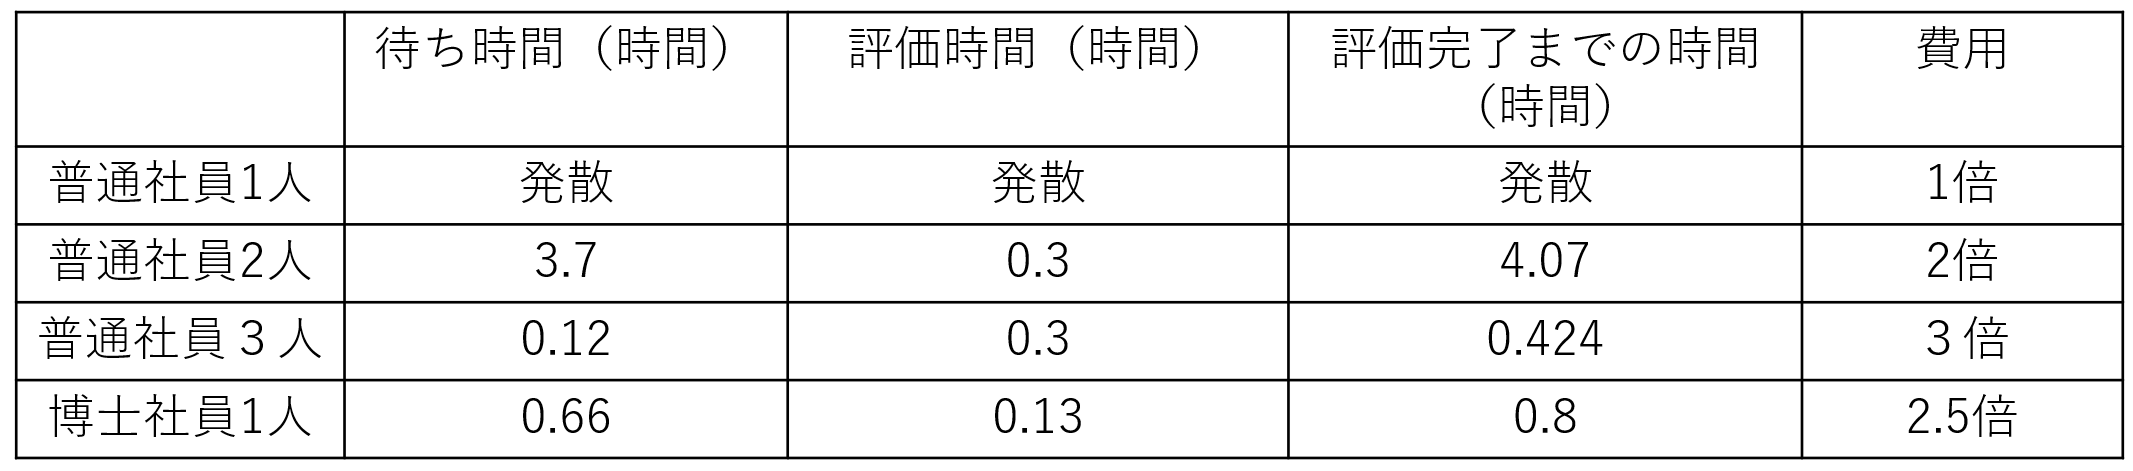
\includegraphics[width=\linewidth]{2.png}}
    \end{figure}
    この場合、結果以上のテーブルとなる。普通社員一人の場合、評価しきれなくなり、系内人数がどんどん伸びて行く。これはどうしても避けてはいけない状況である。
    普通社員2人から普通社員3人や博士社員1人への差は大きい。どれを選ぶかは結局何を重視するか(0.4時間の差が重要か等)は相談して決めることになるだろう。

\end{CJK}


\end{document}
